\chapter{Menü}
\label{cha:menu}

Das Menü untergliedert sich in eine \nameref{sec:menu_navigation} (Kapitel \ref{sec:menu_navigation}) und verschiedenen Übersichts- bzw Schnellzugriffs- Möglichkeiten (Kapitel \ref{sec:menu_approvedservice}, \ref{sec:menu_qualification}, \ref{sec:menu_profile}, \ref{sec:menu_logout}, \ref{sec:menu_applyclient}, \ref{sec:menu_changeclient})

\begin{figure}[h]
 \begin{addmargin}{-0.2\linewidth}
   \centering 
   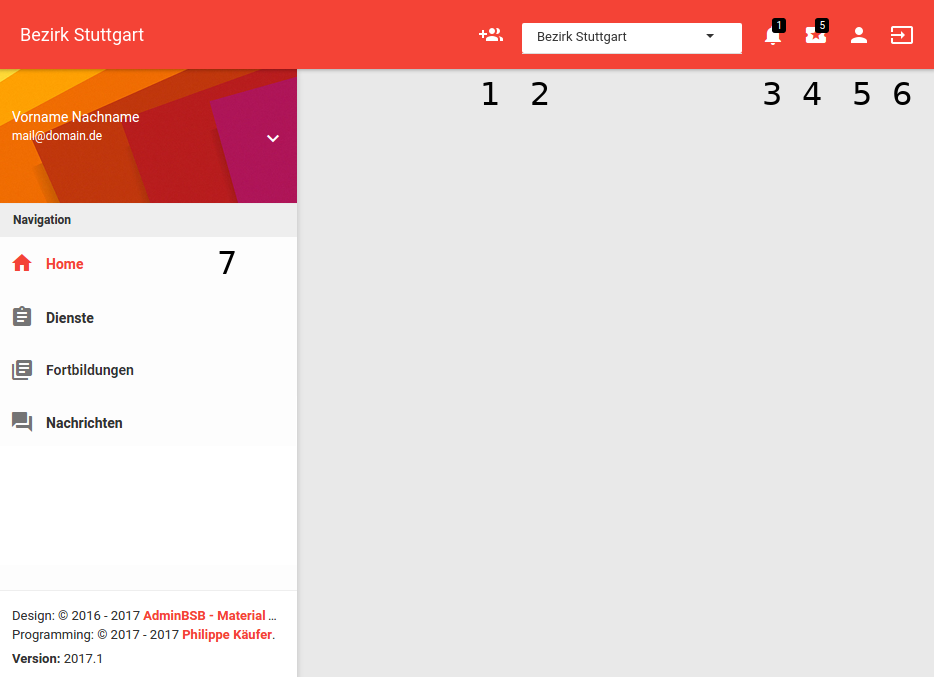
\includegraphics[width=14cm]{Bilder/view_menu.png}
 \end{addmargin} 
 \caption[Menü ansicht]{Dienstplan Menü ansicht}
 \label{fig:view_menu}
\end{figure}

\section{Registrieren für weitere Gliederungen}
\label{sec:menu_applyclient}
Ist ein Benutzer in mehreren Gliederungen tätig, kann er über den Menüpunkt eine Zuordnung zu weiteren Gliederungen beantragen. Die Administratoren der beantragten Gliederung müssen den Antrag bestätigen bevor dem Benutzer Zugriff gewährt wird.

\noindent (Abbildung \ref{fig:view_menu} \textit{\nameref{fig:view_menu}}, Markierung \textit{1})

\section{Wechseln der Gliederungen}
\label{sec:menu_changeclient}
Ist ein Benutzer mehreren Gliederungen zugeordnet, wird eine Dropdown-Liste angezeigt welches ein Wechsel der Ansicht zwischen den Gliederungen ermöglicht. Bei einem Login wird automatisch die zuletzt verwendete Gliederung geladen.

\noindent (Abbildung \ref{fig:view_menu} \textit{\nameref{fig:view_menu}}, Markierung \textit{2})

\section{Zugeteilte Dienste}
\label{sec:menu_approvedservice}
Darstellung als Schnellübersicht der bestätigten Dienste für den jeweiligen Benutzer.

\noindent (Abbildung \ref{fig:view_menu} \textit{\nameref{fig:view_menu}}, Markierung \textit{3})

\section{Eigene Qualifikationen}
\label{sec:menu_qualification}
Darstellung als Schnellübersicht der zugeteilten Qualifikationen für den jeweiligen Benutzer.

\noindent (Abbildung \ref{fig:view_menu} \textit{\nameref{fig:view_menu}}, Markierung \textit{4})

\section{Profil}
\label{sec:menu_profile}
Schnellzugriff auf das Benutzerprofil.

\noindent (Abbildung \ref{fig:view_menu} \textit{\nameref{fig:view_menu}}, Markierung \textit{5})

\vspace*{5mm} \noindent Im Profil kann ein Benutzer seine Daten ändern und auf dem Aktuellsten Stand halten. Wenn die Eingabe des Passwortes leer bleibt wird dieses nicht geändert. Beim erstmaligen Login empfiehlt es sich hier die Handynummer zu hinterlegen.  

\section{Logout}
\label{sec:menu_logout}
Über den Menüpunkt wird der Benutzer abgemeldet.

\noindent (Abbildung \ref{fig:view_menu} \textit{\nameref{fig:view_menu}}, Markierung \textit{6})

\section{Navigation}
\label{sec:menu_navigation}
Aufgrund einer niedrigen Auflösung oder kleineren Displaygröße wird bei manchen Geräten das Menü auf der Linken Seite \noindent (Abbildung \ref{fig:view_menu} \textit{\nameref{fig:view_menu}}, Markierung \textit{7}) nicht dargestellt. Das Menü kann dort über die links oben dargestellten drei Striche ein bzw. ausgeblendet werden.

\noindent Die Navigation enthält bei einem Benutzer folgende Einträge: 
\begin{itemize}
\item \nameref{cha:dashboard} (Kapitel: \ref{cha:dashboard})
\item \nameref{cha:dienste} (Kapitel: \ref{cha:dienste})
\item \nameref{cha:fortbildungen} (Kapitel: \ref{cha:fortbildungen}) \textit{Nur verfügbar, wenn diese für die jeweilige Gliederung freigeschaltet ist.}
\item \nameref{cha:nachrichten} (Kapitel: \ref{cha:nachrichten})

\end{itemize}